\documentclass[11pt,a4paper]{article}

% ── Encodage & langue ──
\usepackage[utf8]{inputenc}
\usepackage[T1]{fontenc}
\usepackage[french]{babel}
\usepackage{lmodern}

% ── Mise en page ──
\usepackage[a4paper,margin=2.3cm,headheight=15pt]{geometry}
\usepackage{xcolor}
\usepackage{titlesec}
\usepackage{enumitem}
\usepackage{booktabs}
\usepackage{array}
\usepackage{fancyhdr}
\usepackage{tabularx}
\usepackage{graphicx}
\usepackage{float}
\usepackage[hidelinks]{hyperref}

% ── Couleurs de la charte ──
\definecolor{primary}{HTML}{1D4ED8}
\definecolor{ink}{HTML}{0F1B2D}
\definecolor{soft}{HTML}{64748B}
\definecolor{line}{HTML}{E2E8F0}
\definecolor{ok}{HTML}{047857}
\definecolor{wip}{HTML}{B45309}
\definecolor{plan}{HTML}{6B7280}
\definecolor{boxbg}{HTML}{F1F5F9}

% ── Titres de sections ──
\titleformat{\section}
  {\color{primary}\large\bfseries}{\thesection.}{0.5em}{}
\titleformat{\subsection}
  {\color{ink}\normalsize\bfseries}{\thesubsection}{0.5em}{}
\titlespacing*{\section}{0pt}{14pt}{6pt}
\titlespacing*{\subsection}{0pt}{8pt}{3pt}

% ── En-tête / pied de page ──
\pagestyle{fancy}
\fancyhf{}
\renewcommand{\headrulewidth}{0.4pt}
\renewcommand{\footrulewidth}{0pt}
\lhead{\small\color{soft}AgentFlow — Rapport d'avancement}
\rhead{\small\color{soft}Fadi Khala}
\cfoot{\small\color{soft}\thepage}

% ── Listes plus compactes ──
\setlist[itemize]{leftmargin=1.4em,itemsep=1.5pt,topsep=2pt}
\setlist[enumerate]{leftmargin=1.6em,itemsep=1.5pt,topsep=2pt}

% ── Étiquettes d'état ──
\newcommand{\etat}[2]{\textbf{\color{#1}#2}}
\newcommand{\fait}{\etat{ok}{Terminé}}
\newcommand{\encours}{\etat{wip}{En cours}}
\newcommand{\planifie}{\etat{plan}{Planifié}}

\begin{document}

% ══════════════════════════════════════════════════════
% EN-TÊTE DU RAPPORT
% ══════════════════════════════════════════════════════
\begin{center}
  {\color{soft}\small RAPPORT D'AVANCEMENT DE PROJET}\\[6pt]
  {\color{ink}\LARGE\bfseries AgentFlow}\\[4pt]
  {\color{primary}\large Plateforme de création et de déploiement d'agents RAG}\\[10pt]
  \color{line}\rule{\linewidth}{0.8pt}
\end{center}

\vspace{2pt}
\noindent
\begin{tabularx}{\linewidth}{@{}l X r@{}}
  \small\color{soft}\textbf{Étudiant :} \small Fadi Khala &
  &
  \small\color{soft}\textbf{Encadrant :} \small Pr. Omri \\
  \small\color{soft}\textbf{Projet :} \small AgentFlow &
  &
  \small\color{soft}\textbf{Date :} \small 13 juillet 2026 \\
\end{tabularx}
\vspace{6pt}

% ══════════════════════════════════════════════════════
\section{Introduction et contexte}

Ce document présente l'état d'avancement du projet \textbf{AgentFlow}, une
plateforme web permettant à une organisation de \emph{construire, configurer,
déployer et exploiter} des agents conversationnels basés sur la technologie
\textbf{RAG} (\emph{Retrieval-Augmented Generation}), à partir de ses propres
documents internes et \textbf{sans écrire de code}.

L'idée centrale est de séparer clairement trois rôles au sein d'une même
organisation :
\begin{itemize}
  \item l'\textbf{Administrateur}, qui gère l'organisation, les départements,
        les utilisateurs et les fournisseurs de modèles (clés API) ;
  \item l'\textbf{ingénieur IT}, qui construit et règle finement les pipelines
        RAG, les teste, puis les déploie ;
  \item l'\textbf{utilisateur final} (\emph{end-user}), qui interroge en langage
        naturel les agents mis à sa disposition et consulte les documents
        sources.
\end{itemize}

La plateforme est multi-organisation et cloisonnée par \textbf{département}
(ex.\ RH, Finance, Juridique), chaque département disposant de ses propres
espaces documentaires et de ses propres agents.

% ══════════════════════════════════════════════════════
\section{Objectifs du projet}

\textbf{Objectif général.} Offrir un outil « no-code » complet qui rend
accessible la mise en place d'un système RAG de qualité professionnelle, tout en
laissant à l'ingénieur IT le contrôle fin de chaque étape du pipeline.

\smallskip
\textbf{Objectifs spécifiques.}
\begin{itemize}
  \item Prendre en charge de multiples sources et formats de documents
        (PDF, DOCX, PPTX, CSV, XLSX, HTML, pages web, Google Drive).
  \item Rendre \emph{chaque} étape du pipeline configurable : découpage
        (\emph{chunking}), vectorisation (\emph{embedding}), recherche et
        génération.
  \item Permettre l'itération : tester plusieurs configurations, les
        sauvegarder en versions, puis déployer la meilleure.
  \item Gérer finement les permissions (propriétaire, collaborateurs IT, accès
        des utilisateurs finaux) et la confidentialité des espaces.
  \item Fournir une expérience utilisateur soignée pour la consultation des
        agents et des documents.
\end{itemize}

% ══════════════════════════════════════════════════════
\section{Méthodologie et organisation du travail}

Le développement suit une démarche \textbf{itérative et incrémentale}, organisée
par lots fonctionnels. Chaque itération livre une fonctionnalité complète et
testée de bout en bout : conception, implémentation côté backend (services et
modèles), implémentation côté frontend (React), puis vérification sur une base de
données réelle.

\begin{itemize}
  \item Versionnement du code avec Git et suivi continu des évolutions.
  \item Migrations de schéma légères et idempotentes, exécutées au démarrage,
        pour faire évoluer la base sans rupture ni outil externe.
  \item Tests de fumée systématiques à chaque étape (permissions, cycle de
        déploiement, accès) sur la base PostgreSQL du projet.
  \item Principe directeur : expérience « no-code » pour l'utilisateur final,
        contrôle complet pour l'ingénieur IT.
\end{itemize}

% ══════════════════════════════════════════════════════
\section{Architecture technique}

Le projet suit une architecture en couches, avec une séparation nette entre les
routes HTTP, la logique métier (\emph{services}) et les modèles de données.

\begin{center}
\renewcommand{\arraystretch}{1.25}
\begin{tabularx}{\linewidth}{@{}>{\bfseries\color{ink}}l X@{}}
  \toprule
  Couche & Technologies et rôle \\
  \midrule
  Frontend & \textbf{React} + \textbf{Vite} — interfaces distinctes par rôle
             (Admin, IT, End-user), design responsive. \\
  Backend  & \textbf{FastAPI} (Python) — API REST, authentification par jeton,
             contrôle d'accès par rôle. \\
  Base de données & \textbf{PostgreSQL} + extension \textbf{pgvector} pour le
             stockage et la recherche vectorielle. \\
  Fournisseurs & \textbf{Groq}, \textbf{OpenAI}, \textbf{Ollama} (LLM),
             \textbf{BGE-M3}/\textbf{Cohere} (embeddings), \textbf{Docling}
             (parsing), \textbf{Crawl4AI} (web), \textbf{Google Drive}. \\
  \bottomrule
\end{tabularx}
\end{center}

La couche « fournisseurs » est entièrement \textbf{modulaire} : chaque famille
(chargeurs, parseurs, nettoyeurs, découpage, embedding, LLM) est isolée derrière
une \emph{factory} qui résout dynamiquement le fournisseur et le modèle à partir
de la configuration de l'espace. Cela permet d'ajouter un fournisseur sans
modifier le reste du code.

% ══════════════════════════════════════════════════════
\section{Modèle de données}

Les principales entités de la base reflètent directement le domaine métier :

\begin{center}
\renewcommand{\arraystretch}{1.25}
\begin{tabularx}{\linewidth}{@{}>{\bfseries\color{ink}}l X@{}}
  \toprule
  Entité & Rôle \\
  \midrule
  Organisation / Département / Utilisateur & Structure multi-organisation et
    rôles (Admin, IT, End-user). \\
  RAGSpace & Configuration complète du pipeline, statut, propriétaire et
    visibilité. \\
  RAGSpaceVersion & Instantané (\emph{snapshot}) d'une configuration ; support du
    versioning et du déploiement. \\
  RAGSpaceCollaborator & IT co-constructeurs autorisés par le propriétaire. \\
  RAGSpaceAccess & Liste des utilisateurs finaux autorisés à interroger un espace
    publié. \\
  Document & Fichier source et son cycle de vie : UPLOADING $\rightarrow$ LOADED
    $\rightarrow$ EXTRACTED $\rightarrow$ INDEXED. \\
  Chunk & Fragment de texte vectorisé, stocké dans pgvector avec ses métadonnées. \\
  \bottomrule
\end{tabularx}
\end{center}

% ══════════════════════════════════════════════════════
\section{Conception}

Cette section illustre, à l'aide de diagrammes de séquence, les principaux
scénarios d'interaction entre l'utilisateur, l'interface, l'API, la base de
données et les modèles.

\subsection{Création d'un espace RAG}
L'ingénieur IT renseigne la configuration ; l'API vérifie ses droits, crée
l'espace (propriétaire, visibilité, statut Brouillon) et enregistre les règles
d'accès.
\begin{figure}[H]
  \centering
  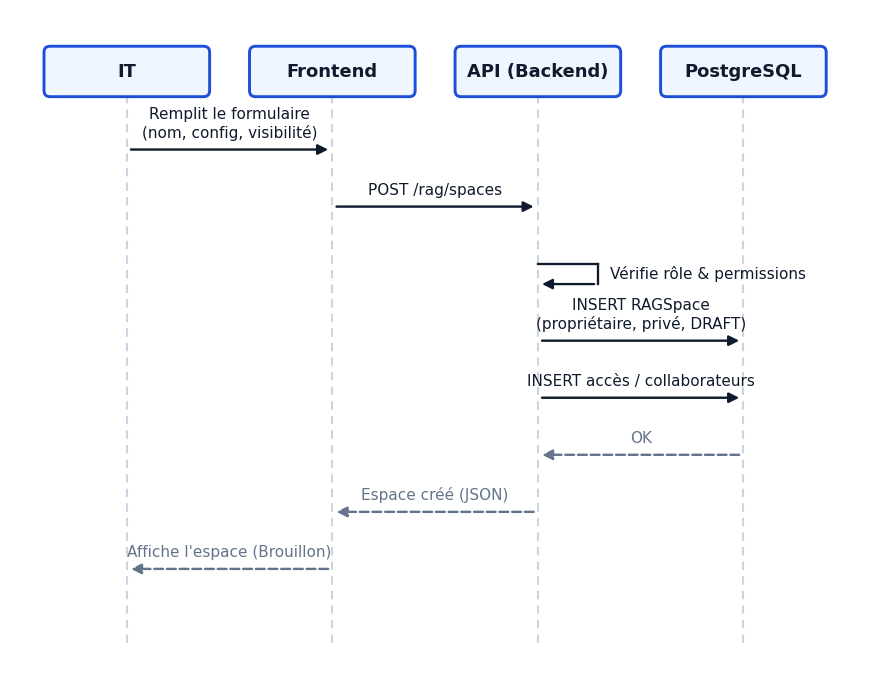
\includegraphics[width=0.82\linewidth]{images/seq_creation.png}
  \caption{Diagramme de séquence — Création d'un espace RAG}
\end{figure}

\subsection{Exécution du système RAG}
À chaque question, l'API contrôle l'accès, vectorise la requête, effectue une
recherche hybride dans pgvector, puis fait générer la réponse par le LLM avec les
passages retrouvés comme contexte.
\begin{figure}[H]
  \centering
  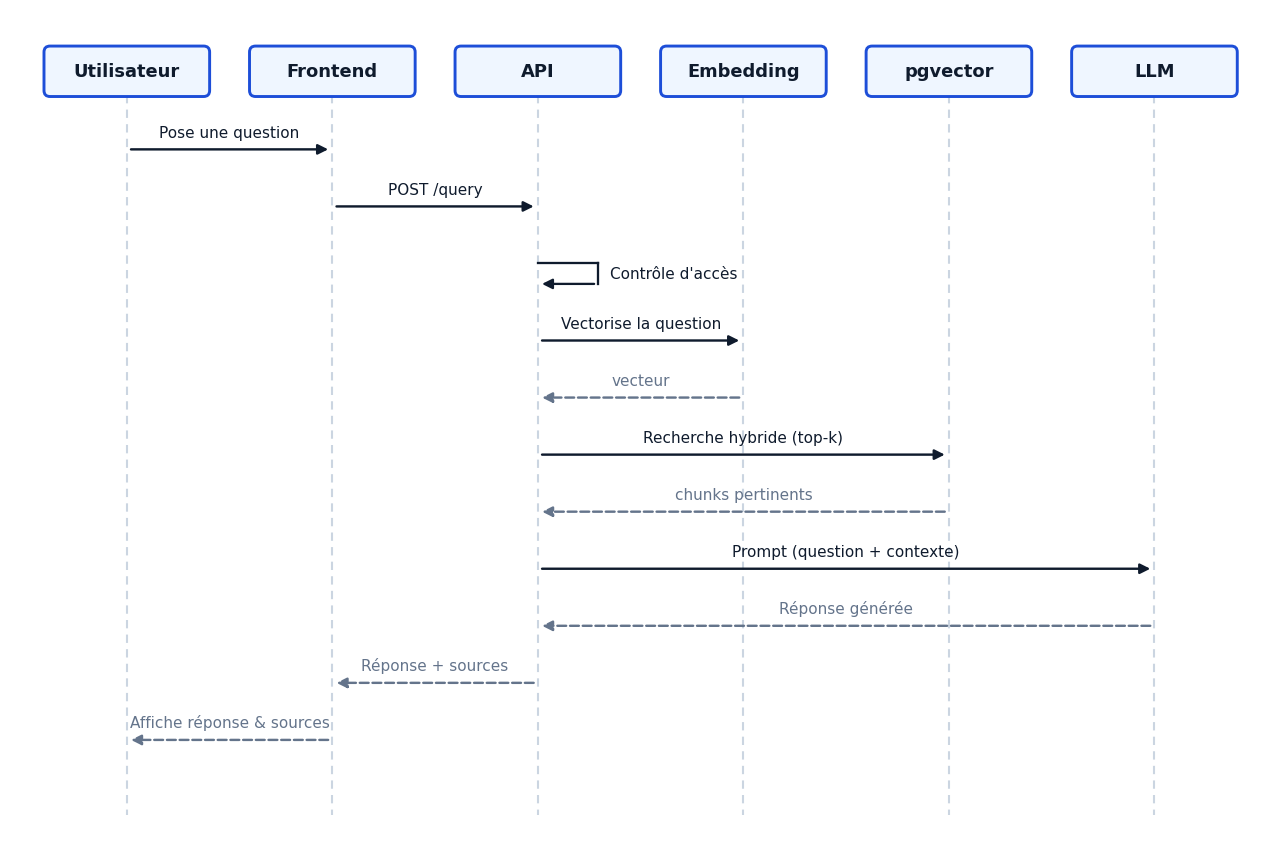
\includegraphics[width=\linewidth]{images/seq_execution.png}
  \caption{Diagramme de séquence — Exécution du système RAG}
\end{figure}

\subsection{Gestion des clés API}
Les clés fournisseurs ne sont jamais stockées en clair : elles sont chiffrées
avant enregistrement, puis déchiffrées uniquement au moment de l'appel au modèle.
\begin{figure}[H]
  \centering
  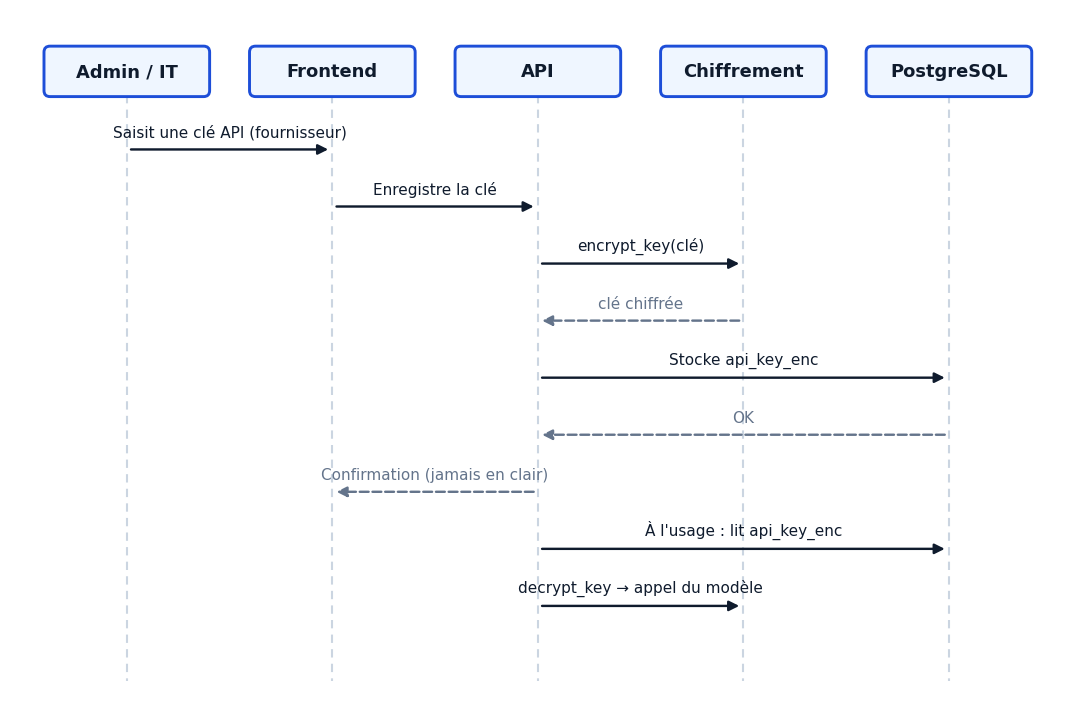
\includegraphics[width=0.82\linewidth]{images/seq_apikey.png}
  \caption{Diagramme de séquence — Gestion des clés API}
\end{figure}

% ══════════════════════════════════════════════════════
\section{Le pipeline RAG (cœur du projet)}

Chaque document parcourt un pipeline complet, dont chaque étape est visualisable
et paramétrable par l'ingénieur IT :

\begin{center}
\renewcommand{\arraystretch}{1.2}
\begin{tabularx}{\linewidth}{@{}>{\bfseries}l X@{}}
  \toprule
  Étape & Description \\
  \midrule
  1. Ingestion   & Import de fichiers, Google Drive, \emph{scraping} d'URL,
                   \emph{crawl} de site, sitemap, flux RSS. \\
  2. Chargement  & Extraction du texte brut et de la structure (Docling pour les
                   PDF/DOCX/PPTX). \\
  3. Nettoyage   & Correction OCR, dé-duplication, masquage des données
                   personnelles (PII). \\
  4. Parsing     & Structuration en sections, tableaux et images ; résumé des
                   images pour les rendre indexables. \\
  5. Découpage   & Stratégies de \emph{chunking} adaptées à chaque format
                   (récursif, par page, par ligne, sémantique, hiérarchique\ldots). \\
  6. Vectorisation & Calcul des \emph{embeddings} (BGE-M3 local par défaut, ou
                   fournisseur externe). \\
  7. Indexation  & Stockage des vecteurs dans pgvector. \\
  8. Recherche   & Recherche \textbf{hybride} (sémantique + mots-clés) avec
                   pondération réglable. \\
  9. Génération  & Réponse produite par le LLM configuré, avec citation des
                   sources et prompt système personnalisable. \\
  \bottomrule
\end{tabularx}
\end{center}

L'ingénieur peut prévisualiser le résultat de chaque étape (texte chargé,
contenu parsé, \emph{chunks} générés) et même \textbf{éditer manuellement} le
contenu extrait avant l'indexation.

% ══════════════════════════════════════════════════════
\section{Travail réalisé}

Cette section présente, captures à l'appui, les étapes clés effectivement
réalisées de la chaîne de traitement.

\subsection{Étape 1 : Extraction de documents}
Le document importé est d'abord chargé (texte brut), puis parsé en une structure
riche : titres, sections, tableaux et images. Le contenu extrait est
prévisualisable et éditable avant l'indexation.
\begin{figure}[H]
  \centering
  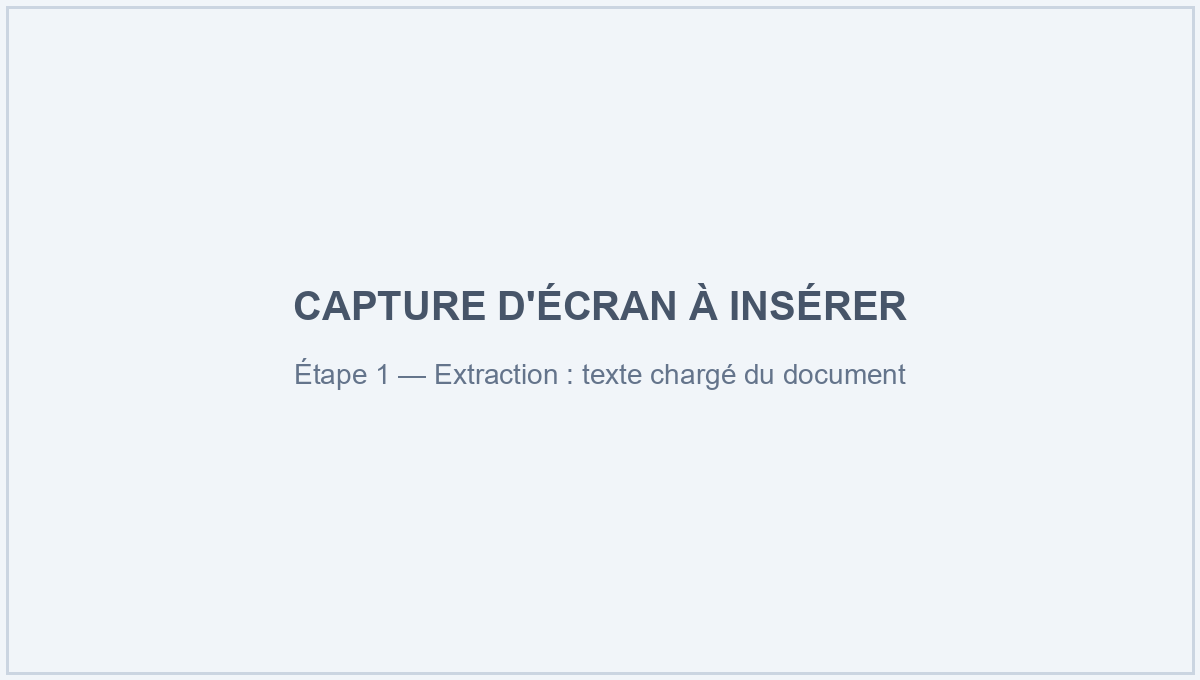
\includegraphics[width=0.8\linewidth]{images/shot_extraction.png}
  \caption{Étape 1 — Extraction : texte chargé du document}
\end{figure}
\begin{figure}[H]
  \centering
  
\includegraphics[width=0.8\linewidth]{images/shot_parsed.png}
  \caption{Étape 1 — Document parsé (sections, tableaux, images)}
\end{figure}

\subsection{Étape 2 : Chunking (découpage)}
Le contenu est découpé en fragments (\emph{chunks}) selon une stratégie adaptée
au format du document, avec des paramètres réglables (taille, chevauchement,
stratégie par format).
\begin{figure}[H]
  \centering
  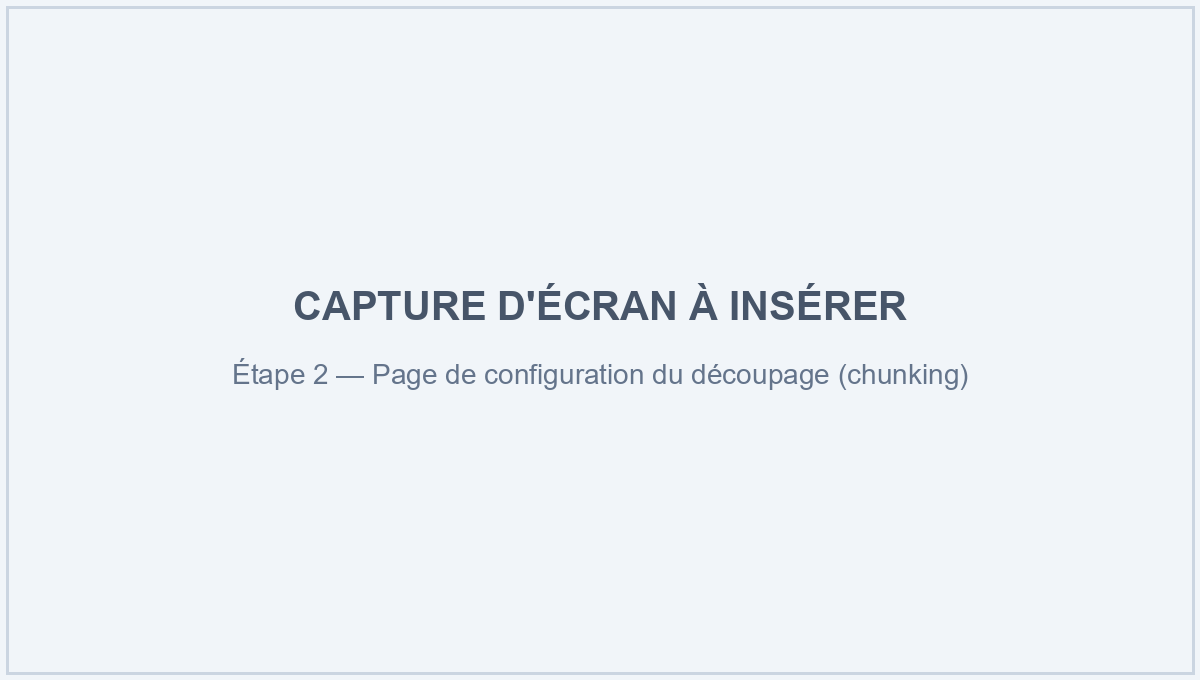
\includegraphics[width=0.8\linewidth]{images/shot_chunking.png}
  \caption{Étape 2 — Page de configuration du découpage}
\end{figure}

\subsection{Étape 3 : Embedding (vectorisation)}
Chaque fragment est transformé en vecteur numérique par un modèle d'embedding
(BGE-M3 local par défaut, ou un fournisseur externe).
\begin{figure}[H]
  \centering
  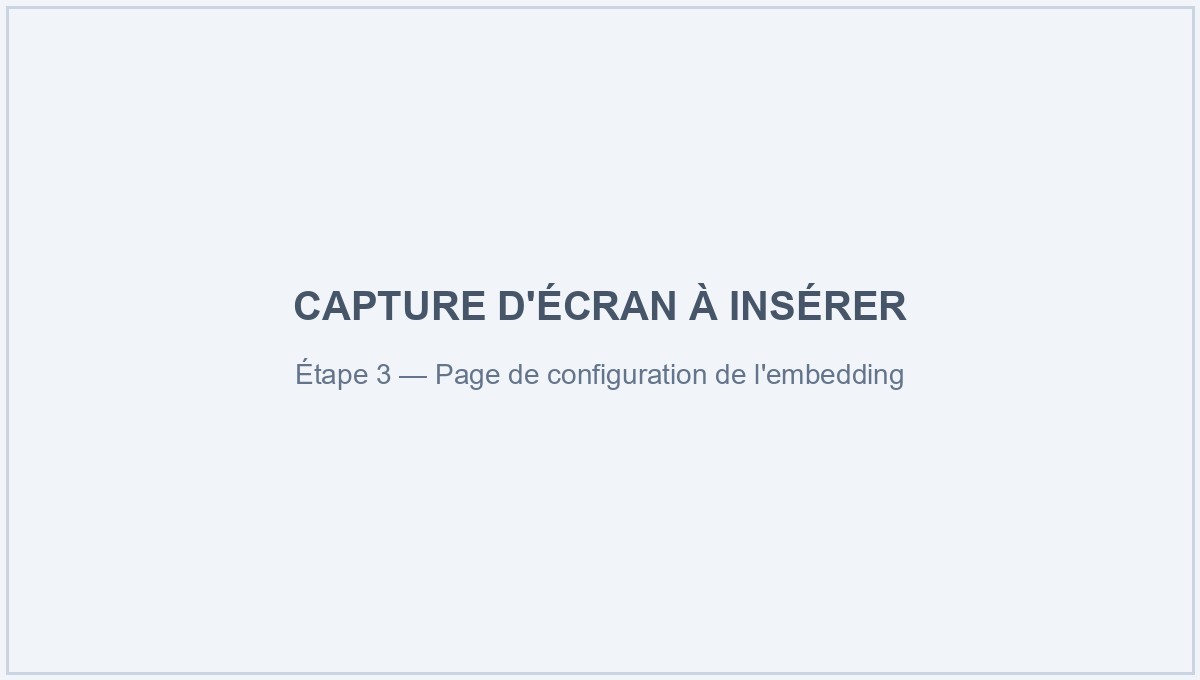
\includegraphics[width=0.8\linewidth]{images/shot_embedding.png}
  \caption{Étape 3 — Page de configuration de l'embedding}
\end{figure}

\subsection{Étape 4 : Stockage vectoriel}
Les vecteurs et leurs métadonnées sont stockés dans PostgreSQL via l'extension
pgvector, avec un index dédié permettant une recherche par similarité efficace.

\subsection{Étape 5 : Recherche hybride}
À l'interrogation, le système combine une recherche sémantique (vecteurs) et une
recherche par mots-clés, avec une pondération réglable, afin de sélectionner les
passages les plus pertinents (top-k).

\subsection{Étape 6 : Génération LLM}
Les passages retrouvés sont fournis comme contexte au modèle de langage choisi,
qui rédige une réponse en citant ses sources. Le fournisseur, le modèle et le
prompt système sont configurables.
\begin{figure}[H]
  \centering
  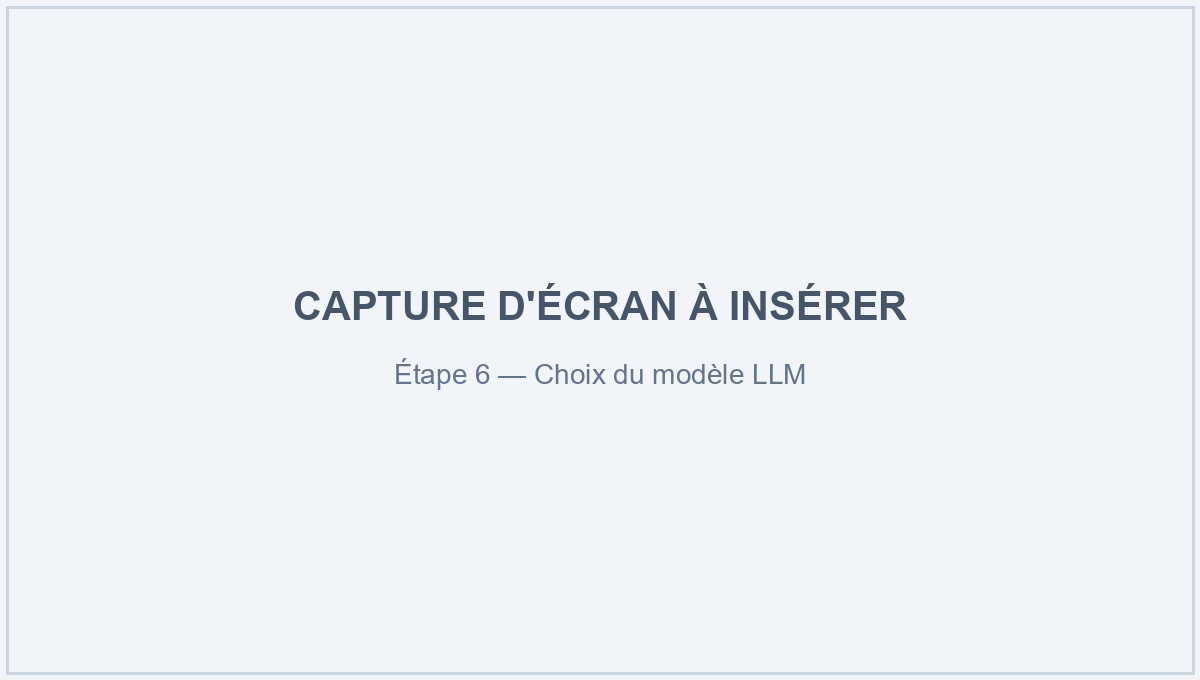
\includegraphics[width=0.8\linewidth]{images/shot_llm.png}
  \caption{Étape 6 — Choix du modèle LLM}
\end{figure}

% ══════════════════════════════════════════════════════
\section{Fonctionnalités réalisées}

\subsection{Gestion des accès et des rôles}
Organisations, départements et utilisateurs avec les rôles Admin / IT /
End-user ; relation \emph{plusieurs-à-plusieurs} entre utilisateurs et
départements ; authentification et invitations.

\subsection{Espaces RAG entièrement configurables}
Création d'un espace rattaché à un département, avec le réglage fin de toutes les
étapes du pipeline (chunking, embedding, LLM, recherche, prompt). Chaque IT peut
utiliser les fournisseurs de l'entreprise ou ses propres clés (chiffrées au
repos).

\subsection{Versioning des configurations et cycle de déploiement}
C'est l'un des apports majeurs de la dernière phase :
\begin{itemize}
  \item l'IT peut \textbf{sauvegarder} plusieurs versions d'une configuration
        (v1, v2\ldots), chacune capturant l'ensemble des paramètres du pipeline ;
  \item il peut \textbf{recharger} une version dans l'éditeur pour la comparer ;
  \item il choisit ensuite la version à \textbf{déployer} auprès des utilisateurs
        finaux.
\end{itemize}
Un cycle de vie clair encadre l'espace : \textbf{Brouillon} $\rightarrow$
\textbf{Déployé} $\rightarrow$ \textbf{En édition}. L'IT peut « mettre en pause »
un agent déployé pour ajouter des documents ou modifier la configuration, puis le
re-déployer ; pendant ce temps, l'utilisateur final voit l'agent avec la mention
« \emph{en mise à jour} ».

\subsection{Détection intelligente de ré-indexation}
Le système distingue les paramètres qui impactent réellement l'index (découpage,
embedding) de ceux qui n'agissent qu'au moment de la requête (LLM, température,
prompt). Une ré-indexation n'est demandée que lorsque la configuration
d'indexation change \emph{effectivement} — l'ajout d'un simple document
n'indexe que ce document, sans reconstruire tout l'index.

\subsection{Modèle de permissions à deux niveaux}
\begin{itemize}
  \item \textbf{Propriétaire} : l'IT créateur de l'espace. Seul à pouvoir
        déployer, publier, importer et supprimer des documents.
  \item \textbf{Collaborateurs IT} : co-constructeurs invités par le
        propriétaire ; ils peuvent régler la configuration, créer des versions et
        tester, mais \emph{pas} déployer ni gérer les documents.
  \item \textbf{Espace privé} : par défaut, un espace n'est visible que de son
        propriétaire et de son équipe IT — aucun utilisateur final n'y accède
        tant qu'il n'est pas explicitement publié.
\end{itemize}

\subsection{Contrôle d'accès des utilisateurs finaux}
Une fois publié, l'accès peut être ouvert à tout le département ou restreint à
une liste précise d'utilisateurs.

\subsection{Expérience utilisateur final}
Interface repensée : liste des agents déployés, conversation en langage naturel
avec citation des sources, et panneau « Documents » permettant d'ouvrir et de
\textbf{consulter les PDF originaux en ligne} (visionneuse intégrée).

\subsection{Prévisualisation IT des agents déployés}
Une vue dédiée permet à l'IT de tester un agent déployé \emph{exactement comme le
voit l'utilisateur final} (même chat, mêmes documents), accessible depuis un menu
« RAG Spaces » à deux entrées : \emph{Espace de travail} et \emph{Agents
déployés}.

% ══════════════════════════════════════════════════════
\section{Synthèse de l'avancement}

\begin{center}
\renewcommand{\arraystretch}{1.3}
\begin{tabularx}{\linewidth}{@{}X l c@{}}
  \toprule
  \textbf{Module} & \textbf{État} & \textbf{Avanc.} \\
  \midrule
  Gestion des utilisateurs / départements / rôles       & \fait      & 100\% \\
  Ingestion multi-source et multi-format                & \fait      & 100\% \\
  Chargement / parsing / nettoyage des documents        & \fait      & 95\%  \\
  Découpage (chunking) par format                       & \fait      & 95\%  \\
  Embeddings et indexation (pgvector)                   & \fait      & 100\% \\
  Recherche hybride et génération (LLM factory)         & \fait      & 95\%  \\
  Versioning et cycle de déploiement                    & \fait      & 90\%  \\
  Permissions (propriétaire / équipe / accès)           & \fait      & 90\%  \\
  Expérience utilisateur final (chat + documents)       & \fait      & 85\%  \\
  Module d'évaluation (comparaison des versions)        & \planifie  & 10\%  \\
  Auto-tuning / découpage agentique                     & \planifie  & 0\%   \\
  Workflows, API Agent, Data Agent                      & \encours   & 30\%  \\
  \bottomrule
\end{tabularx}
\end{center}

\noindent
\textbf{Avancement global estimé : \textasciitilde 80\%.} Le cœur fonctionnel
(pipeline RAG complet, configuration, versioning, déploiement, permissions et
consommation par l'utilisateur final) est opérationnel et testé de bout en bout.

% ══════════════════════════════════════════════════════
\section{Difficultés rencontrées et solutions}

\begin{itemize}
  \item \textbf{Cohérence configuration / index.} Un changement de découpage ou
        d'embedding rend l'index existant obsolète. \emph{Solution} : un
        indicateur de « ré-indexation nécessaire » calculé par \emph{empreinte}
        des seuls paramètres d'indexation, pour n'alerter qu'en cas de
        changement réel.
  \item \textbf{Permissions multi-couches.} Concilier propriétaire,
        collaborateurs IT et accès des utilisateurs finaux sur un même endpoint
        de listing. \emph{Solution} : un filtrage par rôle centralisé dans la
        couche service.
  \item \textbf{Migrations de schéma sans Alembic.} \emph{Solution} : des
        migrations légères et idempotentes exécutées au démarrage
        (\texttt{ADD COLUMN IF NOT EXISTS}, conversion de types).
  \item \textbf{Consultation de fichiers protégés en cross-origin.}
        \emph{Solution} : récupération du fichier en \emph{blob} authentifié côté
        client avant affichage dans la visionneuse.
\end{itemize}

% ══════════════════════════════════════════════════════
\section{Prochaines étapes}

\begin{enumerate}
  \item \textbf{Module d'évaluation} : jeu de test et métriques (taux de
        réponse pertinente, MRR) pour comparer objectivement les versions et
        guider le choix de déploiement.
  \item \textbf{Auto-tuning} : sélection automatique de la stratégie de découpage
        la mieux adaptée à chaque document.
  \item \textbf{Workflows et agents avancés} (API Agent, Data Agent).
  \item \textbf{Historique de conversation} côté utilisateur final.
  \item \textbf{Tests, sécurité et préparation au déploiement} en production.
\end{enumerate}

% ══════════════════════════════════════════════════════
\section{Conclusion}

Le projet AgentFlow a atteint un stade avancé et fonctionnel : l'ensemble de la
chaîne RAG — de l'ingestion des documents jusqu'à la réponse citée à
l'utilisateur final — est en place, avec une gestion complète des
configurations, des versions, du déploiement et des permissions. Les prochaines
étapes se concentreront sur l'\textbf{évaluation quantitative} des
configurations et sur les fonctionnalités avancées, afin de consolider la qualité
et de préparer une mise en production. Je reste à votre disposition pour en
discuter plus en détail lors de la réunion.

\end{document}
